\title{Arjun Trivedi contribution to NIM pub}
\date{June 05, 2014}

\documentclass[12pt]{article}

\usepackage{hyperref}
\usepackage{cite}

\usepackage{graphicx}
%\usepackage{epsfig}
\usepackage{epstopdf}

\begin{document}
\maketitle

% \begin{abstract}
% This is the paper's abstract \ldots
% \end{abstract}

\section{III.E. Photomultiplier tubes (PMTs)}

\subsection{Different PMTs time resolutions}
\textit{My assumptions in writing this section}
\begin{enumerate}
	\item \textit{Our chosen PMT(R9779) was compared with panel-1a PMT(EMI9954A)}
	\item \textit {Details of relevant differences of the tech-specs of the two PMTs and therefore the expected superiority of R9779 over EMI9954A will be listed elsewhere; here we will only give empirical proof}
\end{enumerate}

\textit{By the way, can we use the web link directly to Felician's page as a reference? Perhaps not, but this is just to make a note to confirm this.}

The selected Hamamatusu's R9779 PMTs for panel-1b were compared with Electron Tubes EMI 9954A in the 3-bar setup (\textit{I am assuming that the 3-bar setup will either already be defined or referred to in another publication, so as to not go into details, but simply for the reader to trust that it is our way to extract time-resolution, though, it is NOT directly the time-resolution of the PMT, but of the entire counter; this is important to keep in mind, since for the old TOF system, PMT resolutions were directly compared using lasers; details of this method are in old CLAS-SC NIM paper.})

\textit{Should I mention here that for EMI PMT tests, the contribution of the LFIO module was removed?}

\newpage
Below is the figure that shows the superiority of the R9779:
\begin{figure}[th]
	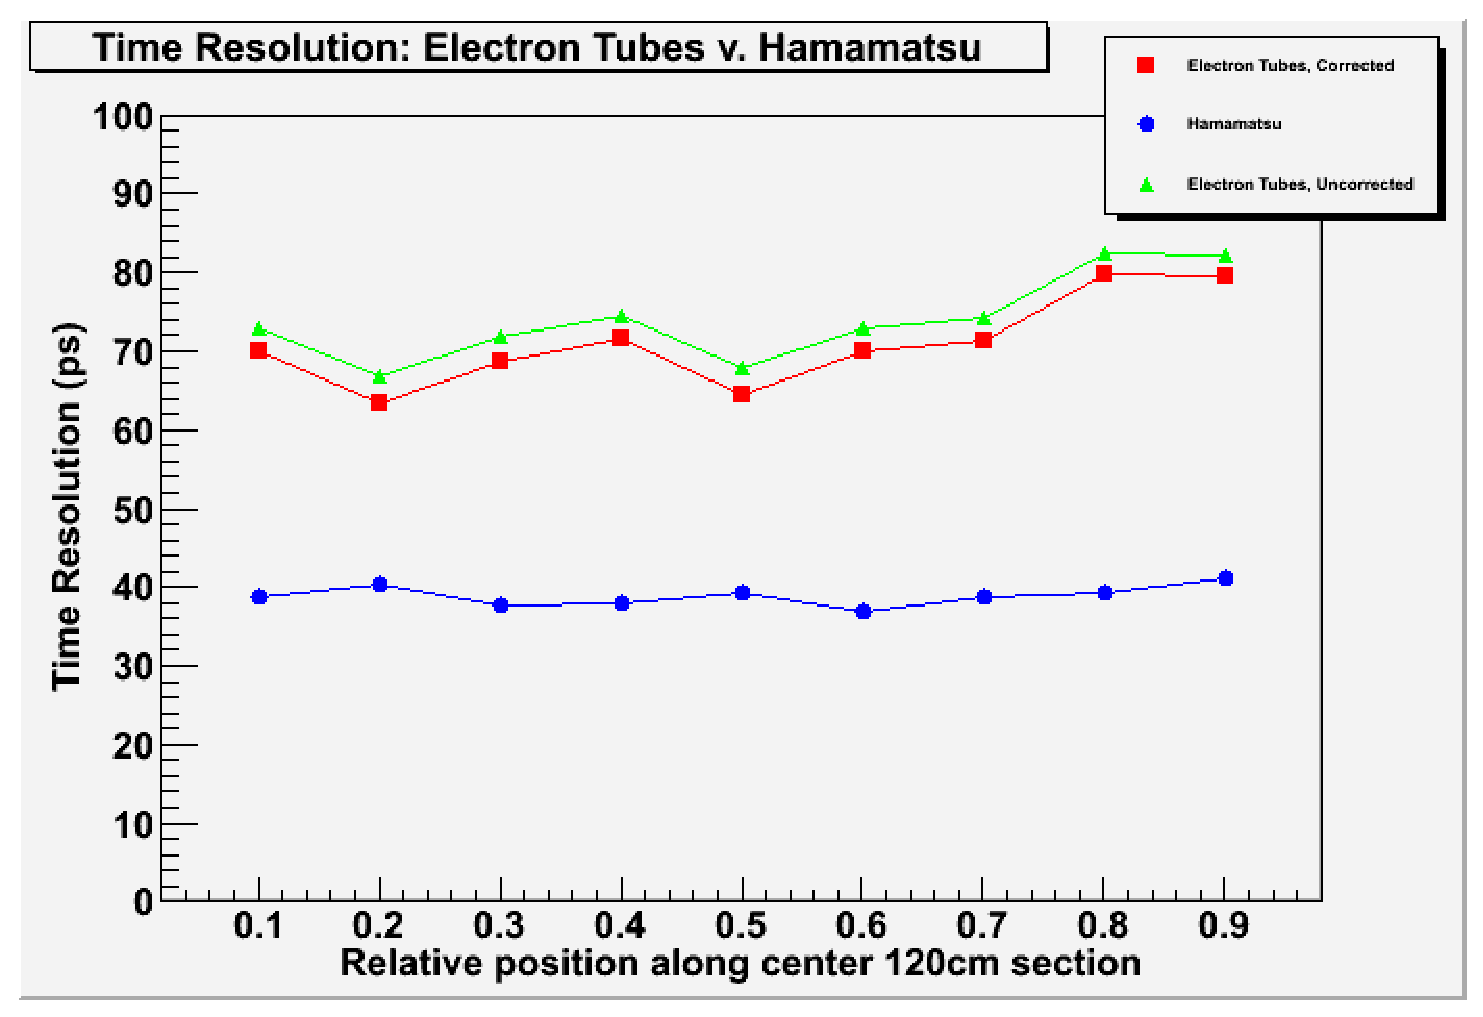
\includegraphics[width=10cm, height=5cm]{PMTcomparison.eps}
\end{figure}

\subsection{... threshold dependence}
\textit{This section is still lazily written}
We also compared various threshold (\textit{Define "threshold"}) levels for the signals from the PMT and see if it had any affect on the time resolution. The threshold levels tried were:50mV, 75mV, 150mV, 300mV, and 600mV.

Following is a figure that demonstrates varying the threshold did not affect the time resolution.
\begin{figure}[th]
	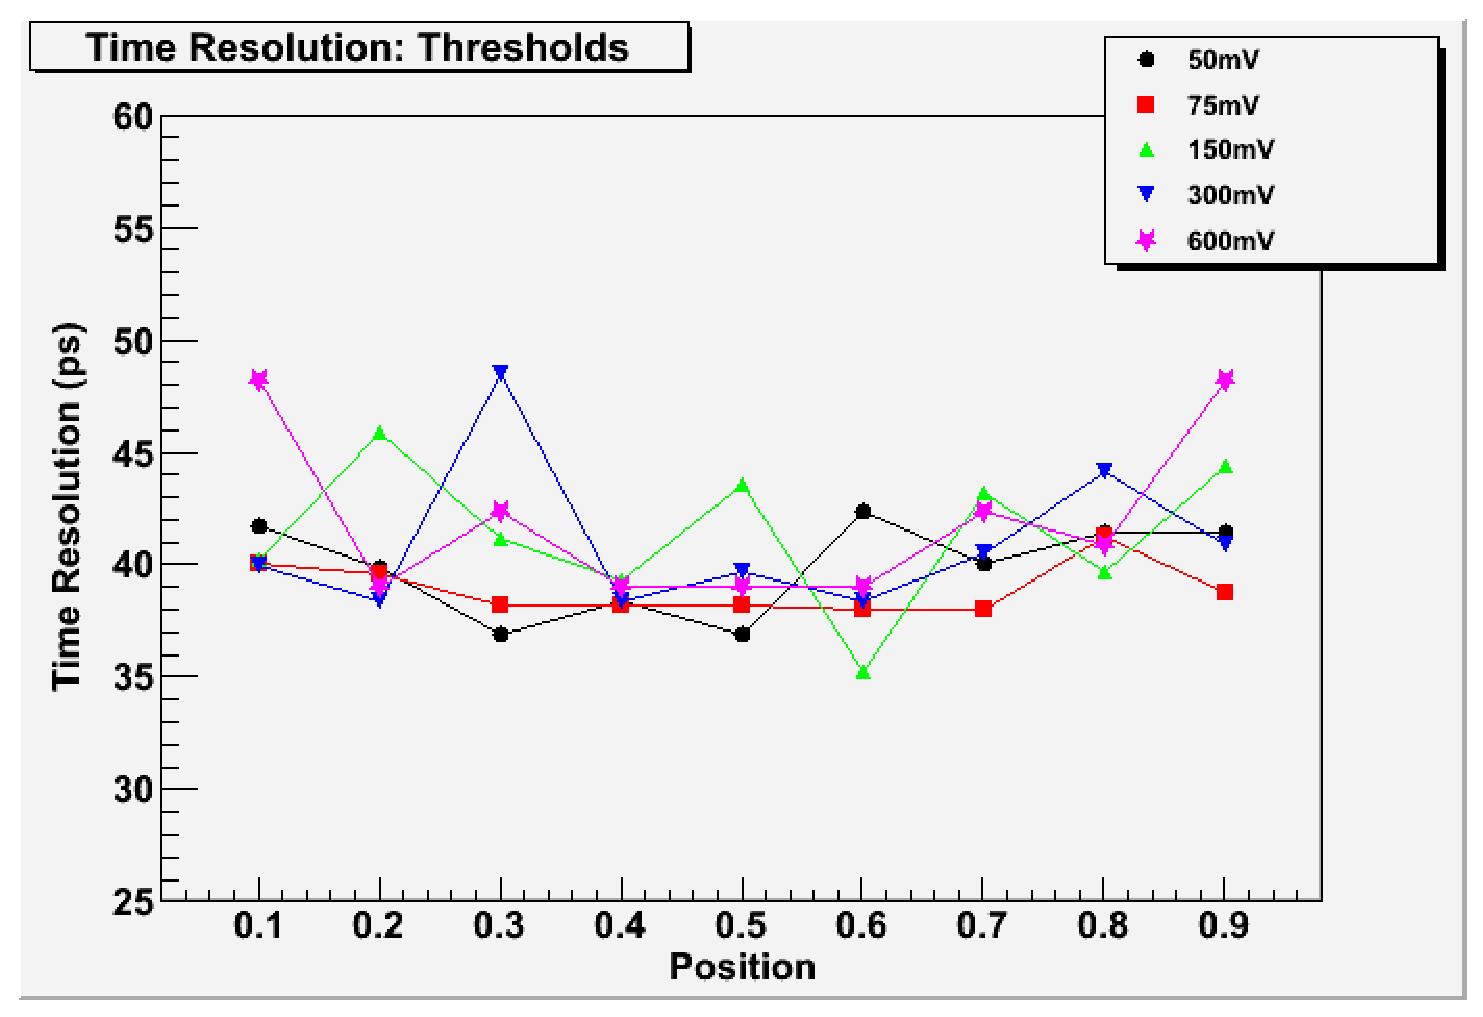
\includegraphics[width=10cm, height=5cm]{ThresholdsTimeRes.eps}
\end{figure}

\section{III.G. Magnetic shielding}
The PMTs that make up the FTOF counters are going to be exposed to the combined magnetic field from the CLAS12 solenoid and torus magnets. It is therefore, important to study the effect of the magnetic field on the signal from the PMT and ultimately, on the time resolution. (\textit{Should I add the following sentence?})It has been qualitatively observed that under such fields, the signal shape is not altered; however the signal amplitude is reduced which depends on the strength of the magnetic field and the PMT's orientation with respect to the field. 

We performed tests to study the response of the PMT signals under varying magnetic field strengths and orientations. It is been observed that when the PMT is transversely aligned to the field (\textit{should define Transverse and Axial and/or illustrate it?}), its signal is most severely affected, as compared to the case when the PMT is axially aligned with the field \cite{Steinman}. Therefore, the PMTs were tested under these orientations to the field, under field strengths varying upto 30G (the maximum field strength that the panel-1b PMTs are going to be exposed to is expected to be 22G, of which 2/3 (15G) will be in the axial direction \cite{CLAS12FTOFstudies})

\textit{Describe and illustrate test set-up}
\begin{itemize}
	\item \textit{Electronics}
	\item \textit{Helmholtz coil}
	\item \textit{Read-out of PMT signal and measure of magnetic field}
\end{itemize}

To begin, the PMTs were tested under 10G-A and 10G-T magnetic fields. Under the 10G-A magnetic field, the signal's ADC mean distribution showed a 10\% reduction; under the 10G-T field, the signal was completely lost \cite{Steinman}.

As a first step, it was decided (\textit{I am not clear about chronological and/or logical steps that led to the final shielding decision: internal mu-metal shielding and external shielding; this may need to be clarified}) to coat the PMTs with a layerof Mu metal, which is a material with very high magnetic permeability,80,000-100,000 (\textit{units}), as compared to a few thousands for steel and therefore, can greatly reduce the affect of the magnetic field without requiring any external shielding \cite{Steinman}. (\textit{Put picture of Mu-metal wrapped PMT from Steinman's thesis?}) After this Mu-metal coating was applied to the PMTs, signal integrity for T fields was intact till 20G; however the A fields on the effect was not altered.

(\textit{Should I mention here Steinman's tests, \cite{Steinman}, that showed that with Mu-metal shielding there was no affect on time resolution upto 20G-T and 10G-A? This is actually all that we would need to sum up this section, since 10G-A is close to the maximum axial field we expect for panel-1b for CLAS12. Actually, what would be better will be obtaining resulutions with our setup in various field configurations as shown in ref \cite{CLAS12FTOFstudies}, where they show a slow, linear reduction in time-resolution of upto 20\% at B=35G-A for 3-inch PMTs and a reduction by 10\% upto 40G for 2-inch PMTs. I feel like our time-resolution will be similar with Mu-metal AND external shielding, but at this point I am unable to scientifically write it down. The closest we can come is to show the integrity of PMT signal upto atleast 30G-A/T, but again with no direct, scientific proof for affects on time-resolution }

(\textit{Since I am not clear on chronology of shielding development, the following paragraph may not be the right way to motivate external shielding and may appear disjointed from the test of the text. In my mind, I think after talking of the effect of Mu-metal shielding, we should use this "rule of thumb" \cite{CLAS12FTOFstudies} in motivation for our choice of external shielding and in the following heirarchical order sum up our results}
\begin{itemize}
	\item \textit{Show the affects of magnetic field on time-resolution in 3-/6-bar method}
	\item \textit{If the above is no longer feasible, then combine Steinman's result, where he showed that upto 10G-A and 20G-T, there was no affect on time-resolution and demonstrate the integrity of the PMT signal, as we tested in South Carolina, to upto 30G-A/T (higher tests needed!)}
\end{itemize})
In reference \cite{CLAS12FTOFstudies}, it is mentioned that "A number of studies have shown that the most effective cylindrical shield for proving performance in an axial field extends past the photocathode by roughly
the diameter of the PMT. In fact, the magnetic shields for the CLAS panel-1a and panel-2 PMTs follow this rule of thumb." Therefore, we employed a rectangular external shielding made up of \textit{X material}, with sides of 2mm thickness and end piece thickness of 5 mm. We tested the shielding for various positions of this external shielding's "over-hang" position as described below:


\subsection{0-,1-,2-,3-cm overhang, axial and transverse, 5-G increments to 30-G}
\textit{Is this needed, if we make the "rule of thumb" argument for our motivation? Perhaps just to confirm that "over-hang" is needed}
\subsection{final shielding and overhang, axial and transverse, 5-G increments to 30-G}
\subsection{time resolution}
\textit{Put results from Steinman's thesis where he showed that time-resolution with Mu-metal and external shielding was maintained till 10G-A and 20G-T}
\subsection{Results and Conclusions}

Given the Mu-metal shielding coating and external shielding, we find that the signal integrity of the PMTs is maintained upto \textit{XX G} and resolutions are unaffected till \textit{YY G}


% \phantomsection
% \addcontentsline{toc}{chapter}{Bibliography}
\label{bib}
\bibliographystyle{abbrv}
\bibliography{at_contrib}

\end{document}